\documentclass[12pt,a4paper]{article}

% -- Packages ------------------------------------------------------------
\usepackage[utf8]{inputenc}
\usepackage[T1]{fontenc}
\usepackage[english]{babel}
\usepackage{geometry}
\geometry{margin=2.5cm, headheight=15pt}
\usepackage{graphicx}
\usepackage{amsmath}
\usepackage{amssymb}
\usepackage{booktabs}
\usepackage{hyperref}
\hypersetup{colorlinks=true, linkcolor=blue, urlcolor=blue, citecolor=blue}
\usepackage{listings}
\usepackage{xcolor}
\usepackage{float}
\usepackage{enumitem}
\usepackage{tikz}
\usetikzlibrary{shapes.geometric, arrows.meta, positioning, fit, backgrounds}
\usepackage{caption}
\usepackage{subcaption}
\usepackage{parskip}
\usepackage{fancyhdr}

% Course code in the header of every page
\pagestyle{fancy}
\fancyhf{}
\fancyhead[R]{SJK009 --- Collaborative Robots}
\fancyfoot[C]{\thepage}
\renewcommand{\headrulewidth}{0.4pt}

% Float placement: pack figures tightly, avoid near-empty pages
\renewcommand{\topfraction}{0.92}
\renewcommand{\bottomfraction}{0.85}
\renewcommand{\textfraction}{0.08}
\renewcommand{\floatpagefraction}{0.75}
\setcounter{topnumber}{3}
\setcounter{totalnumber}{4}

% Last-resort stretch so long monospace paths/topics break instead of overflowing
\setlength{\emergencystretch}{3.5em}

% -- Code style ----------------------------------------------------------
\definecolor{codebg}{RGB}{248,248,248}
\definecolor{codeframe}{RGB}{200,200,200}
\definecolor{keyword}{RGB}{0,100,180}
\definecolor{comment}{RGB}{100,100,100}
\definecolor{string}{RGB}{180,0,0}

\lstset{
  language=Python,
  backgroundcolor=\color{codebg},
  frame=single,
  rulecolor=\color{codeframe},
  basicstyle=\ttfamily\small,
  keywordstyle=\color{keyword}\bfseries,
  commentstyle=\color{comment}\itshape,
  stringstyle=\color{string},
  showstringspaces=false,
  numbers=left,
  numberstyle=\tiny\color{gray},
  numbersep=8pt,
  breaklines=true,
  captionpos=b,
  tabsize=4,
}

% -- TikZ styles ---------------------------------------------------------
\tikzset{
  block/.style={rectangle, draw, fill=blue!10, align=center,
                rounded corners, minimum height=1.2em, minimum width=4cm,
                font=\small},
  sensor/.style={rectangle, draw, fill=green!15, align=center,
                 rounded corners, minimum height=1.2em, minimum width=3.5cm,
                 font=\small},
  decision/.style={diamond, draw, fill=orange!15, align=center,
                   aspect=2, font=\small},
  arrow/.style={->, >=Stealth, thick},
}

% -- Title ----------------------------------------------------------------
\title{%
  \textbf{Person Follower Robot}\\[0.5em]
  \large Sensor Fusion with RGB, Depth, LiDAR, Odometry and Kalman Filter\\[0.3em]
  \normalsize Technical Documentation --- ROS 2 / Webots Simulation
}
\author{Universitat Jaume I}
\date{May 2026}

% ════════════════════════════════════════════════════════════════════════
\begin{document}
\begin{titlepage}
\centering
\vspace*{1.5cm}


\includegraphics[width=0.55\textwidth]{uji_logo.png}

\vspace{1.4cm}
{\large\scshape SJK009 --- Collaborative Robots\par}

\vspace{2.6cm}
{\Huge\bfseries Person Follower Robot\par}
\vspace{0.5cm}
{\large Sensor Fusion with RGB, Depth, LiDAR, Odometry and Kalman Filter\par}
\vspace{0.25cm}
{\normalsize Technical Documentation --- ROS 2 / Webots Simulation\par}

\vspace{2.6cm}
{\large
\renewcommand{\arraystretch}{1.4}
\begin{tabular}{rl}
\textbf{Author:} & Miguel Rebolledo \\
\textbf{Professors:} & Enric Cervera Mateu \\
 & Ángel Juan Durán Bosch \\
\end{tabular}\par}

\vfill
{\large Final Document --- May 2026\par}
\end{titlepage}
\tableofcontents
\newpage

% ════════════════════════════════════════════════════════════════════════
\section{Project Overview}

This document describes the design and implementation of a \textbf{person-following
robot} running on a TurtleBot3 Burger platform~\cite{turtlebot3} inside a
Webots~R2025a simulation~\cite{webots},
controlled through a ROS~2~Humble node~\cite{ros2}.

The system detects a target pedestrian, estimates their position by fusing four
independent sensing modalities, predicts future motion with a Kalman filter, and
commands the robot to follow the person while avoiding obstacles.

\subsection{Goals}
\begin{itemize}
  \item Detect and continuously track a specific person among multiple pedestrians.
  \item Maintain a safe following distance of approximately 0.8~m.
  \item Recover tracking automatically after temporary occlusion or loss of sight.
  \item Avoid collisions using LiDAR-based obstacle detection.
\end{itemize}

\subsection{Software Stack}
\begin{center}
\begin{tabular}{ll}
\toprule
\textbf{Component} & \textbf{Technology} \\
\midrule
Simulation         & Webots R2025a \\
Middleware         & ROS 2 Humble \\
Object detection   & YOLOv8n (Ultralytics) \\
Object tracking    & BoTSORT \\
Depth estimation   & Range Finder (simulated) \\
Laser scanning     & LDS-01 LiDAR \\
Localisation       & Odometry + ArUco markers \\
State estimation   & 2-D Kalman Filter \\
Language           & Python 3 \\
\bottomrule
\end{tabular}
\end{center}

% ════════════════════════════════════════════════════════════════════════
\section{Simulation Environment}

The world file \texttt{turtlebot3\_\allowbreak burger\_\allowbreak pedestrian\_\allowbreak simple.wbt} defines an
indoor office-like environment ($5 \times 10$~m floor) with walls, a door, and
four ArUco marker panels mounted at known world positions.

\subsection{Robot Configuration}

The TurtleBot3 Burger is equipped with the following sensors (defined in the
\texttt{.wbt} world and exposed through the URDF plugin):

\begin{center}
\resizebox{\linewidth}{!}{%
\begin{tabular}{lll}
\toprule
\textbf{Sensor} & \textbf{ROS topic} & \textbf{Resolution / Rate} \\
\midrule
RGB camera      & \texttt{/TurtleBot3Burger/camera/image\_color}              & $640\times480$, FOV $64^{\circ}$ \\
Range finder    & \texttt{/TurtleBot3Burger/range\_finder/range\_image/image} & $640\times480$ depth, 10~Hz \\
LiDAR (LDS-01) & \texttt{/scan}                                               & 360 rays, 5~Hz \\
IMU             & \texttt{/imu}                                                & 20~Hz \\
Odometry        & \texttt{/odom}                                               & continuous \\
\bottomrule
\end{tabular}
}
\end{center}

\subsection{ArUco Markers}

Four ArUco markers~\cite{aruco,aruco2} (DICT\_4X4\_50, IDs 0--3, size 0.3~m) are placed at fixed
world coordinates to provide absolute localisation backup:

\begin{center}
\begin{tabular}{cccc}
\toprule
ID & $x$ (m) & $y$ (m) & $z$ (m) \\
\midrule
0 &  7.5 &  5.0 & 1.2 \\
1 &  8.0 & -5.0 & 1.2 \\
2 & 10.0 &  2.0 & 1.2 \\
3 & 10.0 & -2.0 & 1.2 \\
\bottomrule
\end{tabular}
\end{center}

The PNG textures are generated by \texttt{webots/generate\_aruco\_markers.py},
which applies a horizontal mirror flip to compensate for Webots' internal
texture inversion.

% ════════════════════════════════════════════════════════════════════════
\section{System Architecture}

\subsection{ROS 2 Node Graph}

The entire behaviour is implemented in a single ROS~2 node
(\texttt{PersonFollower}), which subscribes to sensor data and publishes
velocity commands at 10~Hz.

\begin{figure}[htbp]
\centering
\resizebox{\ifdim\width>\linewidth \linewidth\else \width\fi}{!}{%
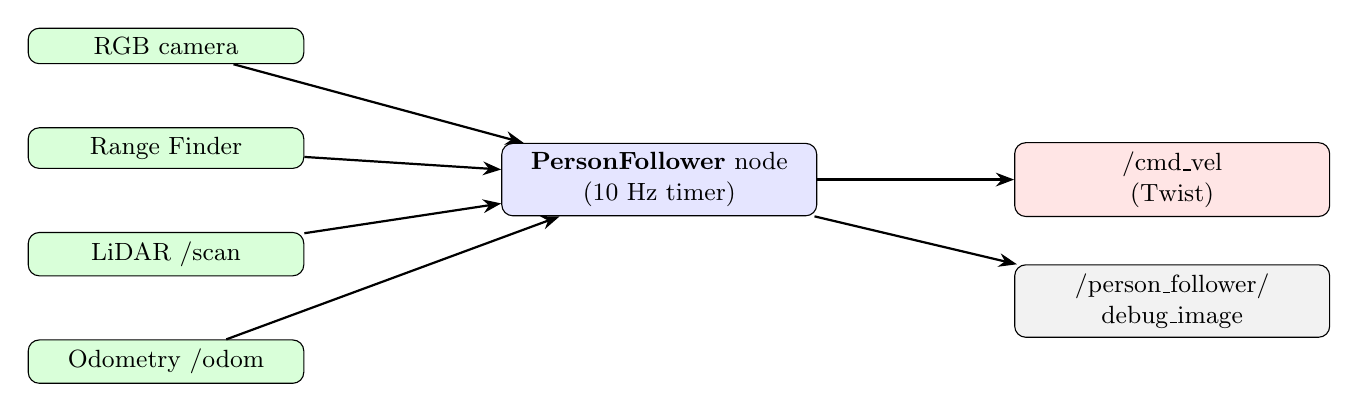
\begin{tikzpicture}[node distance=0.8cm and 2.2cm]
  % Sensor nodes
  \node[sensor] (rgb)   {RGB camera};
  \node[sensor, below=of rgb]   (depth) {Range Finder};
  \node[sensor, below=of depth] (lidar) {LiDAR /scan};
  \node[sensor, below=of lidar] (odom)  {Odometry /odom};

  % Main node
  \node[block, right=2.5cm of depth, yshift=-0.4cm] (pf)
    {\textbf{PersonFollower} node\\(10 Hz timer)};

  % Output
  \node[block, right=2.5cm of pf, fill=red!10] (cmd)
    {/cmd\_vel\\(Twist)};
  \node[block, below=0.6cm of cmd, fill=gray!10] (dbg)
    {/person\_follower/\\debug\_image};

  % Arrows in
  \draw[arrow] (rgb)   -- (pf);
  \draw[arrow] (depth) -- (pf);
  \draw[arrow] (lidar) -- (pf);
  \draw[arrow] (odom)  -- (pf);

  % Arrows out
  \draw[arrow] (pf) -- (cmd);
  \draw[arrow] (pf) -- (dbg);
\end{tikzpicture}%
}
\caption{High-level ROS~2 node graph.}
\end{figure}

\subsection{Processing Pipeline per RGB Frame}

Each incoming RGB frame triggers the following pipeline:

\begin{figure}[htbp]
\centering
\resizebox{\ifdim\width>\linewidth \linewidth\else \width\fi}{!}{%
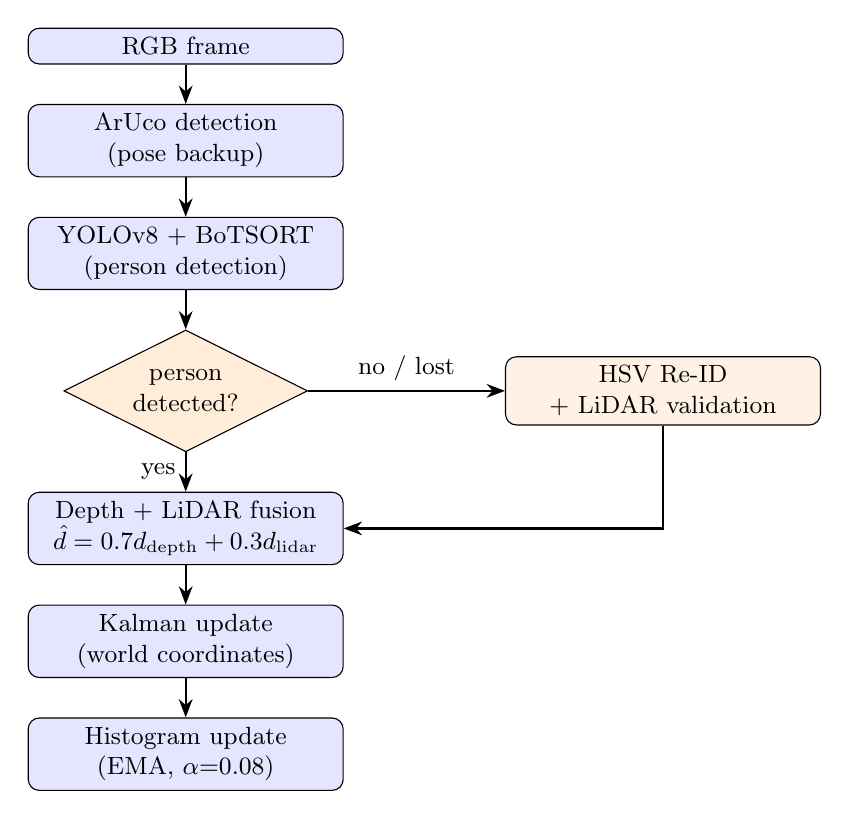
\begin{tikzpicture}[node distance=0.5cm and 0cm, every node/.style={font=\small}]
  \node[block] (in)    {RGB frame};
  \node[block, below=of in]  (aruco) {ArUco detection\\(pose backup)};
  \node[block, below=of aruco] (yolo) {YOLOv8 + BoTSORT\\(person detection)};
  \node[decision, below=of yolo] (det) {person\\detected?};
  \node[block, right=2.5cm of det, fill=orange!10] (reid)
    {HSV Re-ID\\+ LiDAR validation};
  \node[block, below=of det] (fuse) {Depth + LiDAR fusion\\$\hat{d}=0.7d_\text{depth}+0.3d_\text{lidar}$};
  \node[block, below=of fuse] (kal)  {Kalman update\\(world coordinates)};
  \node[block, below=of kal]  (hist) {Histogram update\\(EMA, $\alpha$=0.08)};

  \draw[arrow] (in)    -- (aruco);
  \draw[arrow] (aruco) -- (yolo);
  \draw[arrow] (yolo)  -- (det);
  \draw[arrow] (det)   -- node[left]{yes} (fuse);
  \draw[arrow] (det)   -- node[above]{no / lost} (reid);
  \draw[arrow] (reid)  |- (fuse);
  \draw[arrow] (fuse)  -- (kal);
  \draw[arrow] (kal)   -- (hist);
\end{tikzpicture}%
}
\caption{RGB processing pipeline executed on each camera frame.}
\end{figure}

% ════════════════════════════════════════════════════════════════════════
\section{Software Modules}

\subsection{Camera Model and Intrinsics}

The simulated camera has a horizontal field-of-view of $\text{FOV}_H =
1.117$~rad ($\approx 64^{\circ}$) at resolution $640 \times 480$.  The focal length
in pixels is derived analytically:

\begin{equation}
  f_x = \frac{W/2}{\tan(\text{FOV}_H/2)} \approx 554~\text{px}
\end{equation}

The camera matrix used for ArUco pose estimation, computed with the
OpenCV library~\cite{opencv}, is:
\begin{equation}
  K = \begin{pmatrix} f_x & 0 & W/2 \\ 0 & f_x & H/2 \\ 0 & 0 & 1 \end{pmatrix}
    = \begin{pmatrix} 554 & 0 & 320 \\ 0 & 554 & 240 \\ 0 & 0 & 1 \end{pmatrix}
\end{equation}

Lens distortion is modelled as zero, consistent with the ideal pinhole
camera used in Webots.

\subsection{Kalman Filter (\texttt{KalmanTracker})}

A constant-velocity Kalman filter~\cite{kalman,barshalom} operates in 2-D
world coordinates to
smooth and predict the pedestrian's position. The filter equations are
implemented with NumPy~\cite{numpy}.

\subsubsection*{State vector}
\[
  \mathbf{x} = [x,\; y,\; v_x,\; v_y]^{\top}
\]

\subsubsection*{Transition matrix (variable $\Delta t$)}
\[
  F = \begin{pmatrix}
    1 & 0 & \Delta t & 0 \\
    0 & 1 & 0 & \Delta t \\
    0 & 0 & 1 & 0 \\
    0 & 0 & 0 & 1
  \end{pmatrix}
\]

\subsubsection*{Observation model}
\[
  H = \begin{pmatrix} 1 & 0 & 0 & 0 \\ 0 & 1 & 0 & 0 \end{pmatrix}
\]
Only position $(x, y)$ is observed; velocities are inferred from the filter.

\subsubsection*{Noise matrices}
\[
  Q = \mathrm{diag}(0.05,\; 0.05,\; 0.20,\; 0.20), \quad
  R = 0.3 \cdot I_2
\]

\subsubsection*{Prediction step}
\begin{align}
  \hat{\mathbf{x}}^{-} &= F\,\mathbf{x} \\
  P^{-} &= F\,P\,F^{\top} + Q
\end{align}

\subsubsection*{Update step}
\begin{align}
  \mathbf{y} &= \mathbf{z} - H\,\hat{\mathbf{x}}^{-} \\
  S &= H\,P^{-}\,H^{\top} + R \\
  K &= P^{-}\,H^{\top}\,S^{-1} \\
  \mathbf{x} &\leftarrow \hat{\mathbf{x}}^{-} + K\,\mathbf{y} \\
  P &\leftarrow (I - K\,H)\,P^{-}
\end{align}

\subsubsection*{Future position prediction}
The method \texttt{get\_predicted(t\_ahead)} returns a forward-extrapolated
estimate used to navigate towards the target when vision is temporarily lost:
\[
  (x_\text{pred},\, y_\text{pred}) = (x + v_x\,\tau,\;\; y + v_y\,\tau), \quad \tau = 0.8~\text{s}
\]

\subsection{LiDAR Processing}

\subsubsection*{Obstacle detection}
All LiDAR rays within $\pm30^{\circ}$ of the forward direction are scanned for
finite readings; the minimum value is stored as \texttt{obstacle\_front}.
This is used in the control law to modulate speed.

\subsubsection*{Leg cluster detection (\texttt{\_detect\_leg\_clusters})}
Consecutive LiDAR points closer than 0.15~m (gap threshold) are grouped.
This clustering is a lightweight heuristic variant of laser-based people
detection~\cite{arras}.
A cluster is accepted as a potential human leg if:
\begin{itemize}
  \item It contains between 3 and 12 points.
  \item Its bounding box width is less than 0.35~m.
  \item Its range is less than 2.5~m.
\end{itemize}
The centroid of each accepted cluster is returned in the robot frame.
These centroids are used for two purposes: (1) validating YOLO detections,
and (2) providing an independent distance estimate.

\subsection{Person Detection and Tracking (\texttt{\_process\_yolo})}

\begin{enumerate}[leftmargin=*, label=\arabic*.]
  \item \textbf{YOLO inference.} \texttt{YOLOv8n}~\cite{yolo,yolov8} runs with \texttt{persist=True}
    and the \texttt{botsort.yaml}~\cite{sort,botsort} tracker, returning bounding boxes with stable
    integer track IDs for class~0 (person) with confidence $\geq 0.30$.

  \item \textbf{Target acquisition.} On first detection, the robot locks onto
    the largest bounding box (by area), stores its track ID, and computes an
    initial HSV appearance histogram.

  \item \textbf{Target maintenance.} On subsequent frames the locked ID is
    searched in the result list. If found, the bounding box is used directly.

  \item \textbf{Re-identification (Re-ID).} If the target ID disappears for
    more than 2~s, each currently visible person is compared against the
    stored HSV appearance histogram~\cite{comaniciu} via histogram correlation.  The best candidate is
    accepted if its similarity exceeds 0.75 \emph{and} a LiDAR cluster exists
    within $\pm25^{\circ}$ of its image position.

  \item \textbf{Histogram maintenance.} While the target is at 1--3~m, the
    stored histogram is updated with an exponential moving average:
    \[
      H \leftarrow 0.92\,H + 0.08\,H_\text{new}
    \]
\end{enumerate}

\subsection{Distance Fusion}

Once a bounding box is confirmed, the target distance $\hat{d}$ is computed
by fusing the depth camera and the LiDAR:

\begin{enumerate}
  \item \textbf{Depth camera.} A 25\%-inset ROI of the bounding box is
    sampled from the \texttt{32FC1} depth image.  The median of all valid
    pixels ($0.1 < d < 10$~m) is taken as $d_\text{depth}$.

  \item \textbf{LiDAR.} The nearest leg cluster within $\pm15^{\circ}$ of the
    target heading gives $d_\text{lidar}$.

  \item \textbf{Weighted fusion:}
    \[
      \hat{d} = \begin{cases}
        0.7\,d_\text{depth} + 0.3\,d_\text{lidar} & \text{both available} \\
        d_\text{depth} & \text{depth only} \\
        d_\text{lidar} & \text{LiDAR only} \\
        \text{None}    & \text{neither available}
      \end{cases}
    \]

  \item \textbf{World-coordinate conversion.} When a fused distance is
    available it is converted to world coordinates and fed to the Kalman
    filter:
    \[
      t_x = r_x + \hat{d}\cos(\psi + \theta), \quad
      t_y = r_y + \hat{d}\sin(\psi + \theta)
    \]
    where $(r_x,r_y)$ is the robot position from odometry, $\psi$ is the
    robot yaw, and $\theta$ is the horizontal bearing to the target derived
    from the image column:
    \[
      \theta = \left(\frac{c_x}{W} \cdot 2 - 1\right) \cdot \frac{\text{FOV}_H}{2}
    \]
\end{enumerate}

% ════════════════════════════════════════════════════════════════════════
\section{Control Law}

The control callback runs at 10~Hz and selects one of three operating modes.

\subsection{Obstacle Speed Factor}

Before any movement command is issued, a speed scaling factor is computed
from the frontal LiDAR reading:

\begin{equation}
  s = \begin{cases}
    0 & d_\text{front} < 0.40~\text{m} \\
    0.3 + 0.7\,\dfrac{d_\text{front} - 0.40}{0.65 - 0.40} & 0.40 \le d_\text{front} < 0.65~\text{m} \\
    1 & d_\text{front} \ge 0.65~\text{m}
  \end{cases}
\end{equation}

\subsection{Mode 1: Direct Following (Person Visible)}

When both $\theta$ (bearing) and $\hat{d}$ (distance) are known:

\begin{align}
  \omega &= \text{clip}\!\left(-1.4\,\theta,\; [-\omega_\text{max},\,\omega_\text{max}]\right) \\
  f_a    &= \max\!\left(0,\; 1 - \frac{|\theta|}{\pi/4}\right) \\
  v      &= s \cdot \text{clip}\!\left(0.5\,(\hat{d} - d_\text{des}) \cdot f_a,\;
             [-v_\text{max},\, v_\text{max}]\right)
\end{align}

where $d_\text{des} = 0.8$~m, $v_\text{max} = 0.15$~m/s,
$\omega_\text{max} = 0.6$~rad/s.  If $\hat{d} < d_\text{des}$ the robot
backs up at $-0.10$~m/s.  The factor $f_a$ reduces forward speed when the
robot is turning sharply, preventing it from driving past the target.

\subsubsection*{Mode 1b: Bearing only (no distance)}
When only $\theta$ is available, the robot rotates to face the target and
advances at maximum speed scaled by $f_a$ and $s$.

\subsection{Mode 2: Kalman Dead-Reckoning}

When the person is not currently visible but the Kalman filter is initialised,
the robot navigates to the predicted position $(\hat{x}, \hat{y})$:

\begin{align}
  d_\text{goal}    &= \sqrt{(\hat{x}-r_x)^2 + (\hat{y}-r_y)^2} \\
  \alpha_\text{goal} &= \text{atan2}(\hat{y}-r_y,\;\hat{x}-r_x) - \psi \\
  v   &= \min(v_\text{max}\cdot s,\; 0.3\,d_\text{goal}) \\
  \omega &= \text{clip}(0.8\,\alpha_\text{goal},\; [-\omega_\text{max},\,\omega_\text{max}])
\end{align}

If the robot is within 0.5~m of the predicted point or has been in Kalman
mode for more than 8~s without regaining sight of the target, it switches to
a slow rotation to search (Mode~3) and resets the tracker state.

\subsection{Mode 3: Search Rotation}

The robot spins in the last observed angular direction at 0.3~rad/s until a
person is detected again.

\begin{figure}[htbp]
\centering
\resizebox{\ifdim\width>\linewidth \linewidth\else \width\fi}{!}{%
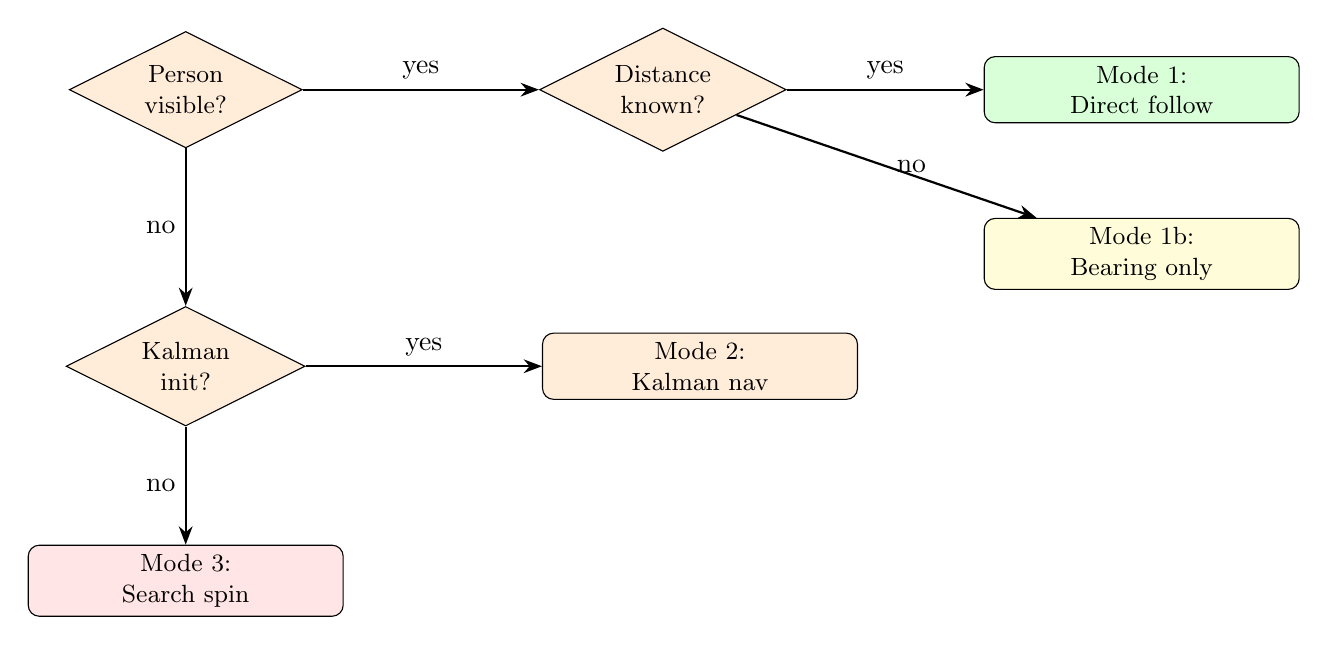
\begin{tikzpicture}[node distance=0.7cm and 1.5cm]
  \node[decision] (vis) {Person\\visible?};
  \node[decision, right=3cm of vis] (dist) {Distance\\known?};
  \node[block, right=2.5cm of dist, fill=green!15] (m1) {Mode 1:\\Direct follow};
  \node[block, below=1.2cm of m1, fill=yellow!15] (m1b) {Mode 1b:\\Bearing only};
  \node[decision, below=2cm of vis] (kal) {Kalman\\init?};
  \node[block, right=3cm of kal, fill=orange!15] (m2) {Mode 2:\\Kalman nav};
  \node[block, below=1.5cm of kal, fill=red!10] (m3) {Mode 3:\\Search spin};

  \draw[arrow] (vis)  -- node[above]{yes} (dist);
  \draw[arrow] (vis)  -- node[left]{no}   (kal);
  \draw[arrow] (dist) -- node[above]{yes} (m1);
  \draw[arrow] (dist) -- node[right]{no}  (m1b);
  \draw[arrow] (kal)  -- node[above]{yes} (m2);
  \draw[arrow] (kal)  -- node[left]{no}   (m3);
\end{tikzpicture}%
}
\caption{Control mode selection logic.}
\end{figure}

% ════════════════════════════════════════════════════════════════════════
\section{ArUco Localisation Backup}

At every RGB frame, the ArUco detector (\texttt{DICT\_4X4\_50}) searches for
known markers.  For each detected marker with known world position
$\mathbf{m}_w$, the pose of the robot is estimated as:

\begin{align}
  d       &= \|\mathbf{t}\|,\quad
  \alpha  = \text{atan2}(t_x, t_z) \\
  \psi_m  &= \text{atan2}(-n_x, n_z) \\
  \phi    &= \psi_m + \alpha - \pi \\
  r_x     &= m_{w,x} + d\cos\phi, \quad r_y = m_{w,y} + d\sin\phi
\end{align}

where $\mathbf{t}$ is the translation vector from the marker pose estimation
and $\mathbf{n} = R_{cm}[:,2]$ is the marker's normal direction.  This
alternative robot position estimate can be used to detect and correct odometry
drift (currently logged at DEBUG level).

% ════════════════════════════════════════════════════════════════════════
\section{Debug Visualisation}

The node publishes a debug image on
\texttt{/person\_\allowbreak follower/\allowbreak debug\_image} combining:
\begin{itemize}
  \item Bounding boxes for all detected persons (green for the target,
    red for others) with track IDs.
  \item Orange dots along the bottom edge indicating the projected
    positions of LiDAR leg clusters.
  \item A text overlay showing obstacle distance, Kalman velocity estimate,
    and current mode (\texttt{SIGUIENDO} / \texttt{RECUPERANDO}).
\end{itemize}

% ════════════════════════════════════════════════════════════════════════
\section{File Structure}

{\small
\begin{verbatim}
person_follower/
+-- person_follower/
|   +-- __init__.py
|   +-- person_follower.py        # Main ROS 2 node (perception + control)
+-- webots/
|   +-- turtlebot3_burger_pedestrian_simple.wbt   # Simulation world
|   +-- turtlebot3_burger_pedestrian_no_walls.wbt # Alternative world
|   +-- generate_aruco_markers.py                 # ArUco PNG generator
|   +-- record_experiment.bash                    # rosbag recording helper
|   +-- aruco_0.png ... aruco_3.png               # Marker textures
|   +-- config.rviz                               # RViz configuration
+-- report/
|   +-- person_follower_report.tex   # This document
|   +-- plot_trajectories.py         # Trajectory plotting / analysis script
|   +-- traj_*.png                   # Generated trajectory figures
|   +-- sim_*.png                    # Simulation screenshots
+-- yolov8n.pt                    # Pre-trained YOLOv8 nano weights
+-- package.xml                   # ROS 2 package manifest
+-- setup.py / setup.cfg          # Python package setup
+-- README.md                     # Build and run instructions
+-- .gitignore
\end{verbatim}
}

% ════════════════════════════════════════════════════════════════════════
\section{Parameter Summary}

\begin{center}
\begin{tabular}{lll}
\toprule
\textbf{Parameter} & \textbf{Value} & \textbf{Description} \\
\midrule
\texttt{desired\_distance}       & 0.80 m   & Target following distance \\
\texttt{max\_linear\_speed}      & 0.15 m/s & Maximum forward/backward speed \\
\texttt{max\_angular\_speed}     & 0.60 rad/s & Maximum rotation speed \\
\texttt{OBSTACLE\_STOP}          & 0.40 m   & Full stop threshold \\
\texttt{OBSTACLE\_SLOW}          & 0.65 m   & Speed ramp threshold \\
\texttt{KALMAN\_TIMEOUT}         & 8.0 s    & Max time in Kalman-only mode \\
\texttt{REID\_MIN\_LOST\_SECS}   & 2.0 s    & Min lost time before Re-ID \\
\texttt{HIST\_MATCH\_THRESHOLD}  & 0.75     & HSV correlation threshold \\
\texttt{ARUCO\_MARKER\_SIZE}     & 0.30 m   & Physical marker side length \\
Depth-LiDAR fusion weight        & 70\%/30\%& Depth preferred over LiDAR \\
\bottomrule
\end{tabular}
\end{center}

% ════════════════════════════════════════════════════════════════════════
\section{Simulation Evidence}

This section presents screenshots taken during live simulation runs in Webots~R2025a,
demonstrating the end-to-end operation of the person-follower system.

\subsection{Simulation World and Pedestrians}

\begin{figure}[htbp]
  \centering
  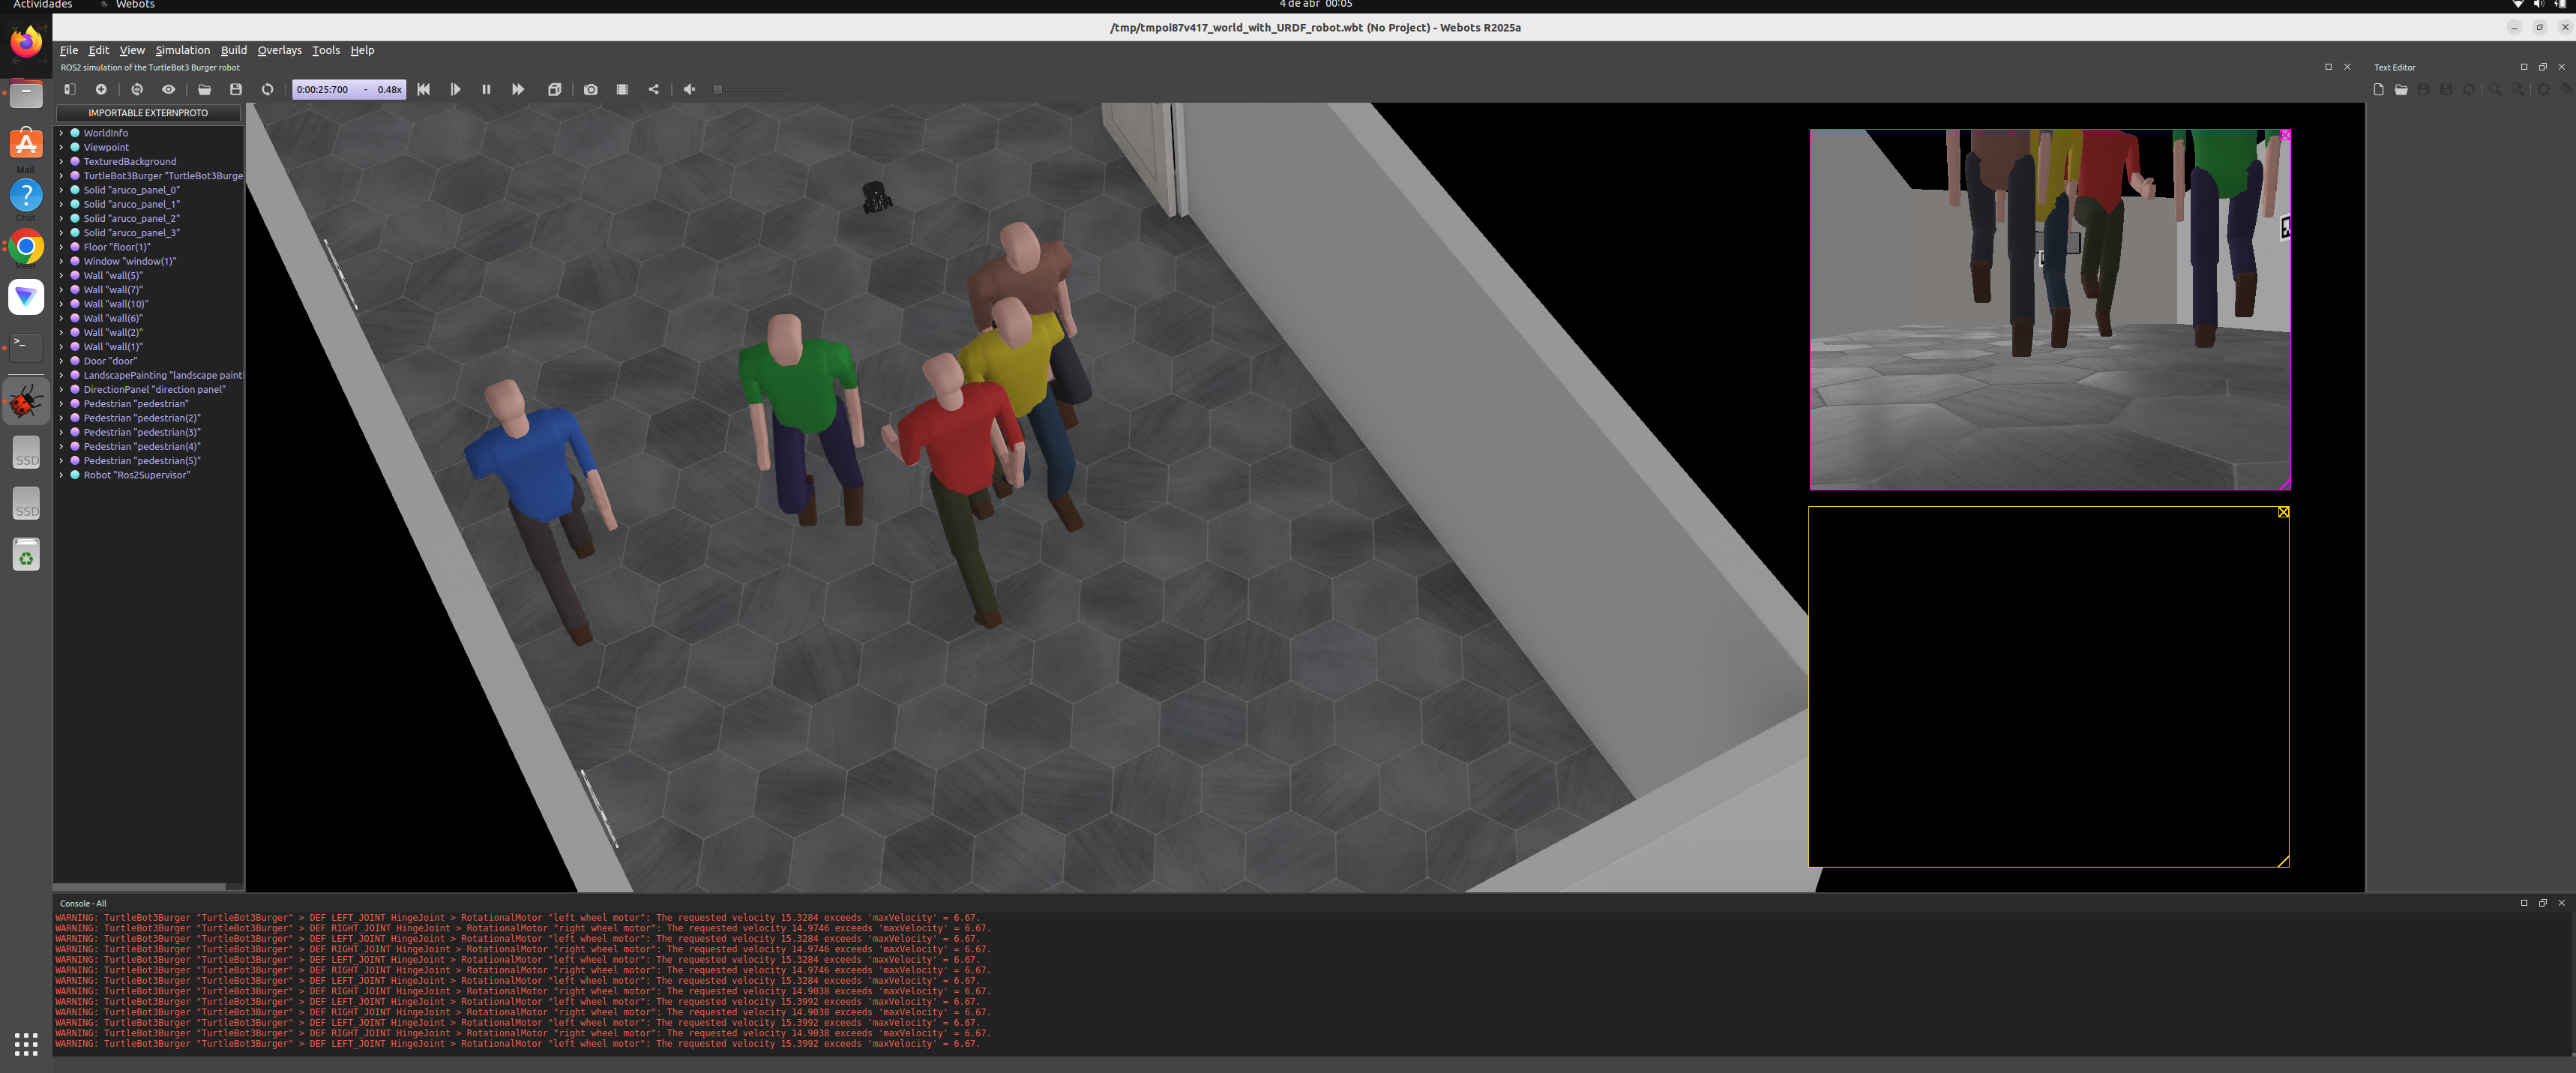
\includegraphics[width=\linewidth,height=0.82\textheight,keepaspectratio]{sim_01_world.png}
  \caption{Webots simulation world with multiple pedestrians. The top-right inset
           shows the robot's onboard RGB camera stream. Several animated pedestrians
           move through the indoor environment while the TurtleBot3 Burger (visible
           in the centre of the scene) prepares to track a target.}
  \label{fig:sim_world}
\end{figure}

\subsection{Active Tracking with Kalman Filter}

\begin{figure}[htbp]
  \centering
  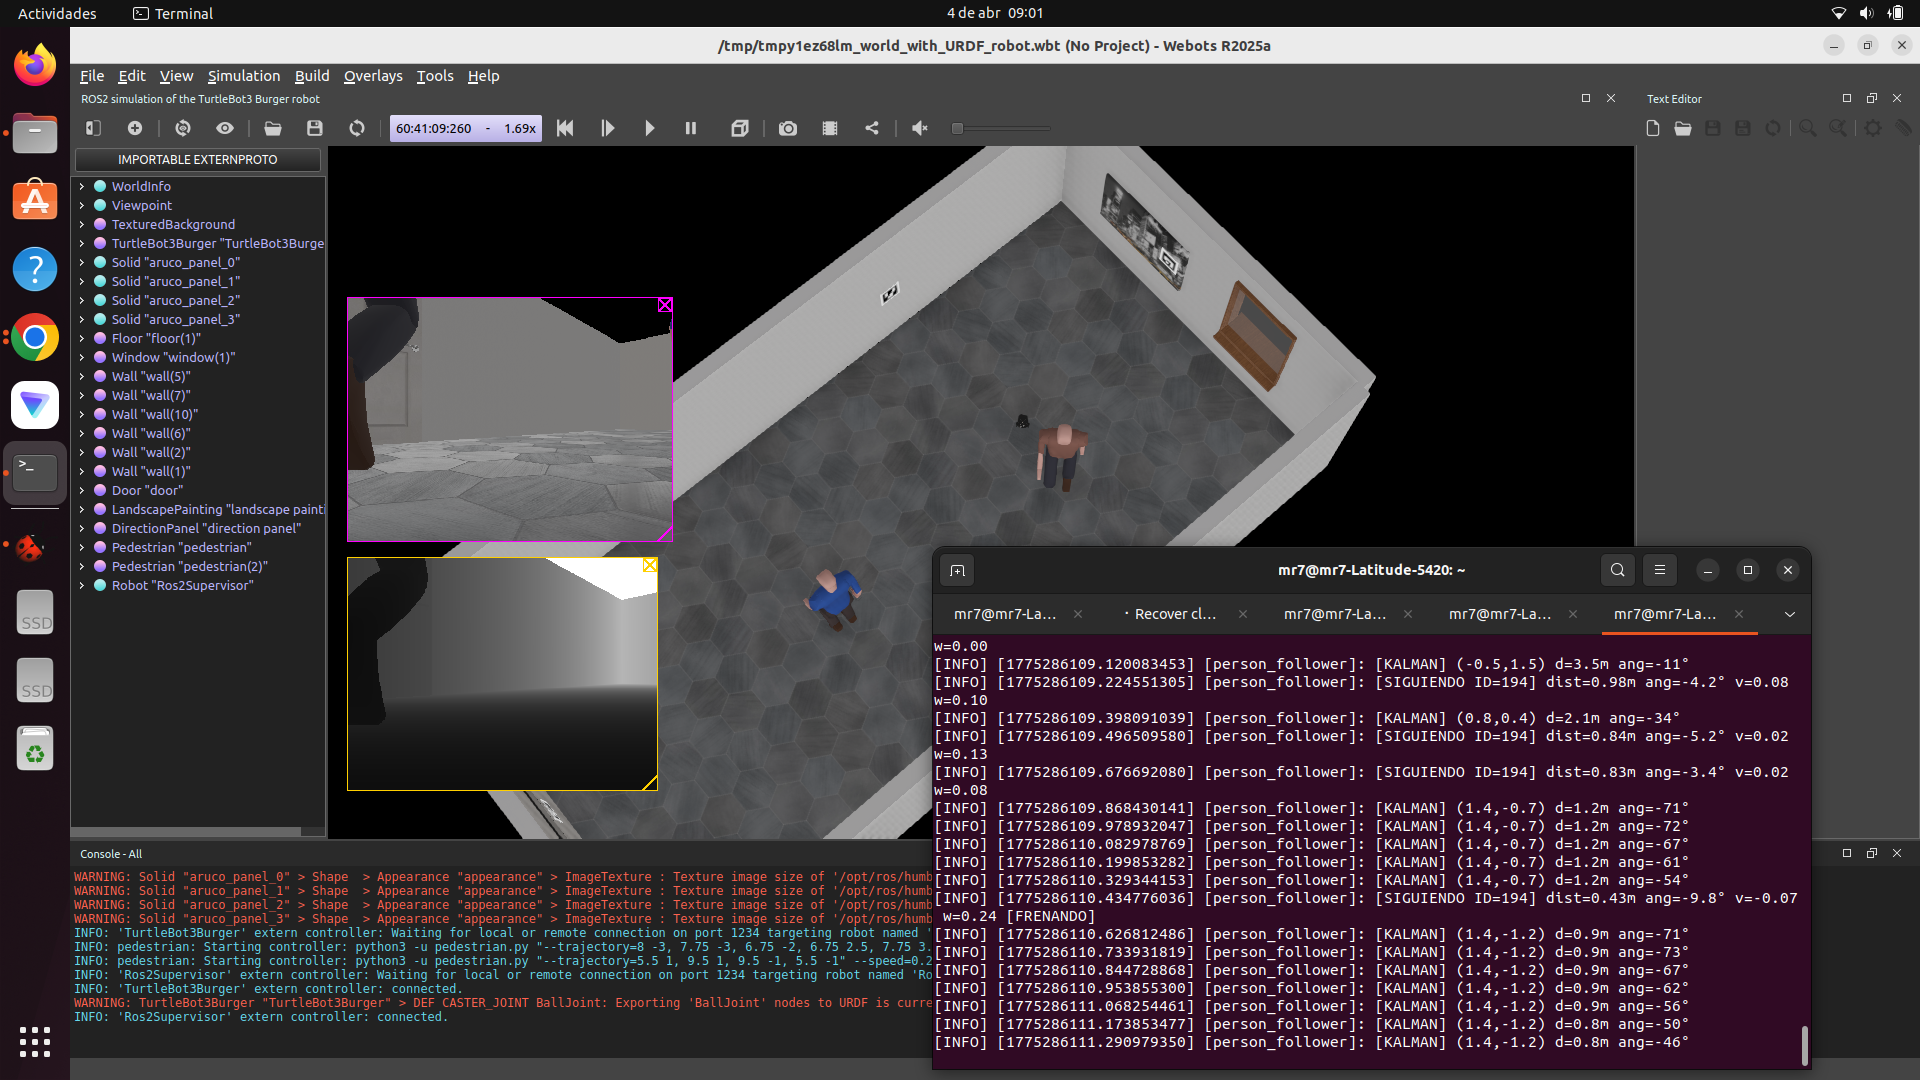
\includegraphics[width=\linewidth,height=0.82\textheight,keepaspectratio]{sim_02_following.png}
  \caption{Robot actively following the locked target. The terminal on the right
           shows ROS~2 log output from the \texttt{person\_follower} node:
           \texttt{[SIGUIENDO ID=94]} entries confirm that the YOLO+BoTSORT
           pipeline has acquired a stable track, and \texttt{[KALMAN]} lines
           show the Kalman filter operating in dead-reckoning mode during
           momentary occlusions. Distance and bearing values are updated at
           10~Hz.}
  \label{fig:sim_following}
\end{figure}

\subsection{Active ROS 2 Topics}

\begin{figure}[htbp]
  \centering
  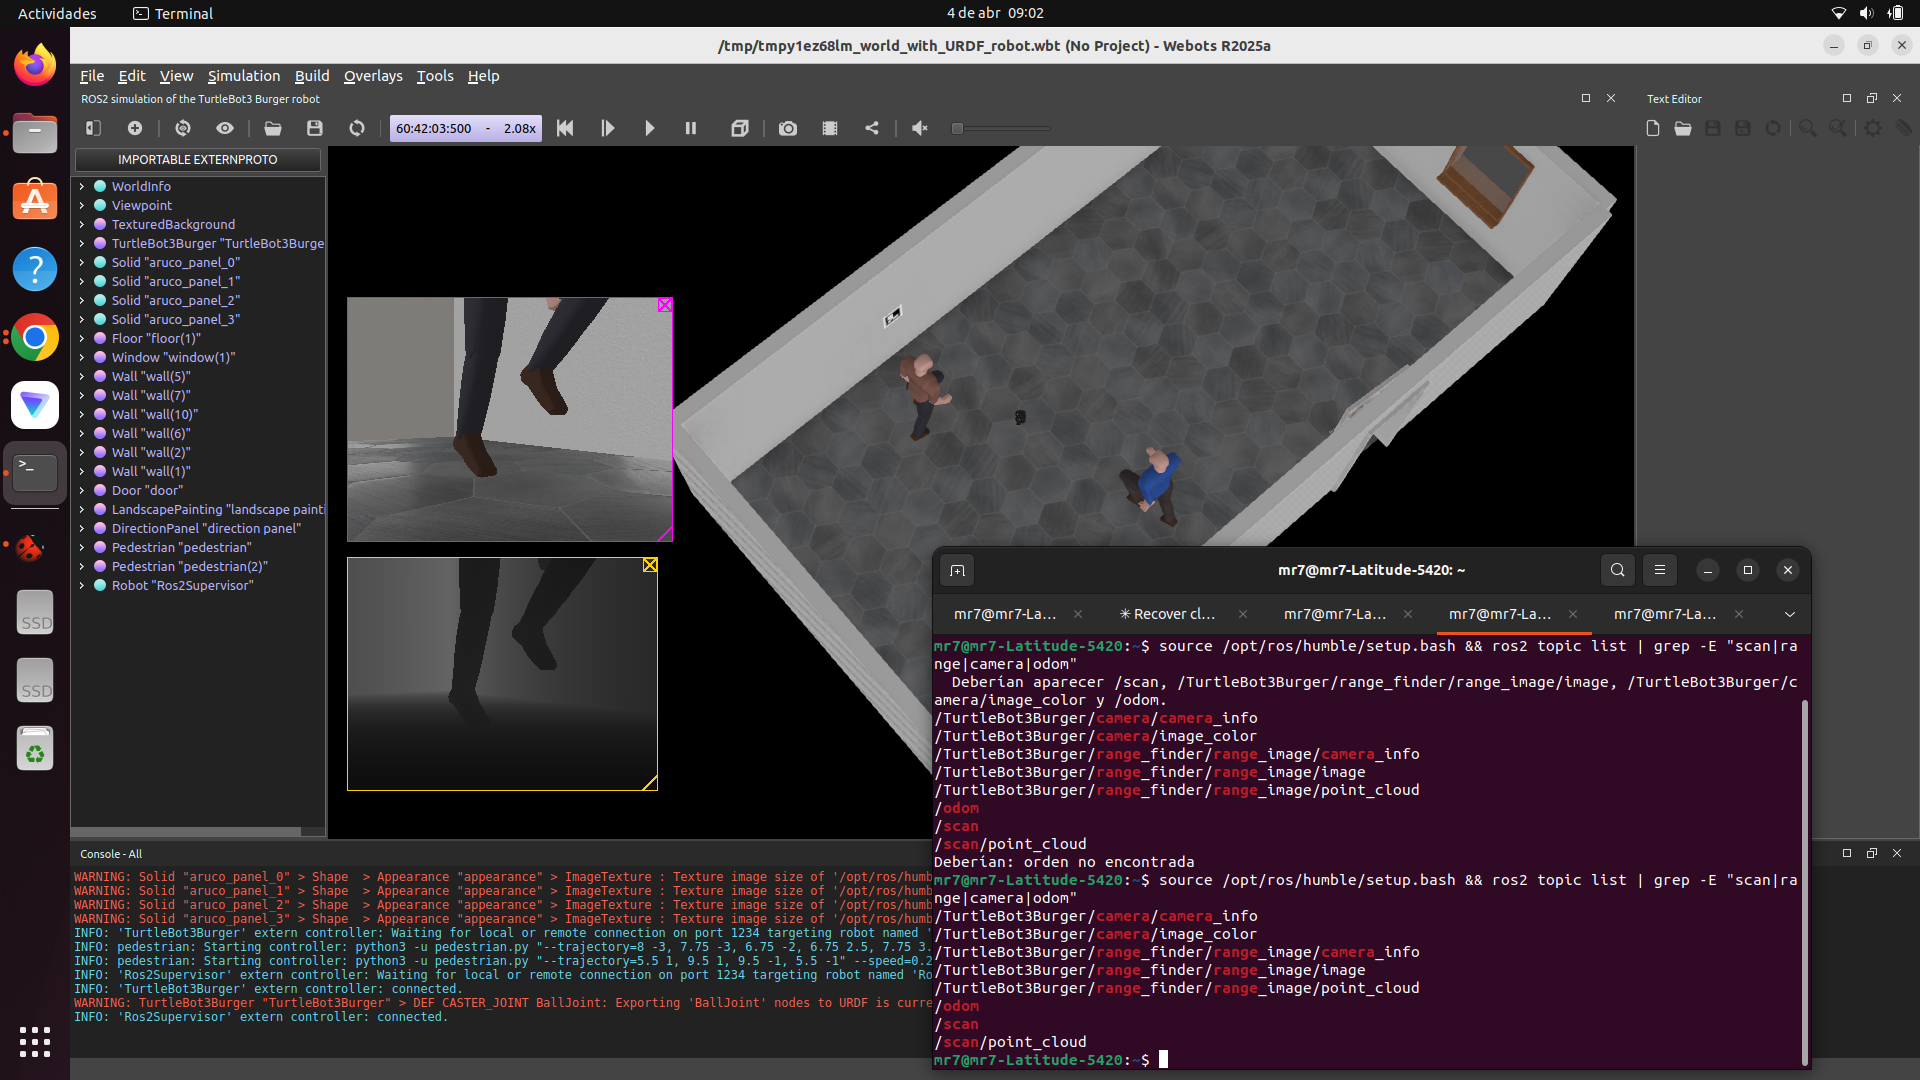
\includegraphics[width=\linewidth,height=0.82\textheight,keepaspectratio]{sim_03_topics.png}
  \caption{ROS~2 topic listing during a live run. All expected sensor streams
           are present: \texttt{/scan} (LiDAR), \texttt{/TurtleBot3Burger/camera/image\_color}
           (RGB), \texttt{/TurtleBot3Burger/range\_finder/range\_image/image} (depth),
           and \texttt{/scan/point\_cloud}. The camera stream also exposes a
           \texttt{/image\_color} sub-topic used internally by the node.}
  \label{fig:sim_topics}
\end{figure}

\subsection{Debug Image and Depth View}

\begin{figure}[htbp]
  \centering
  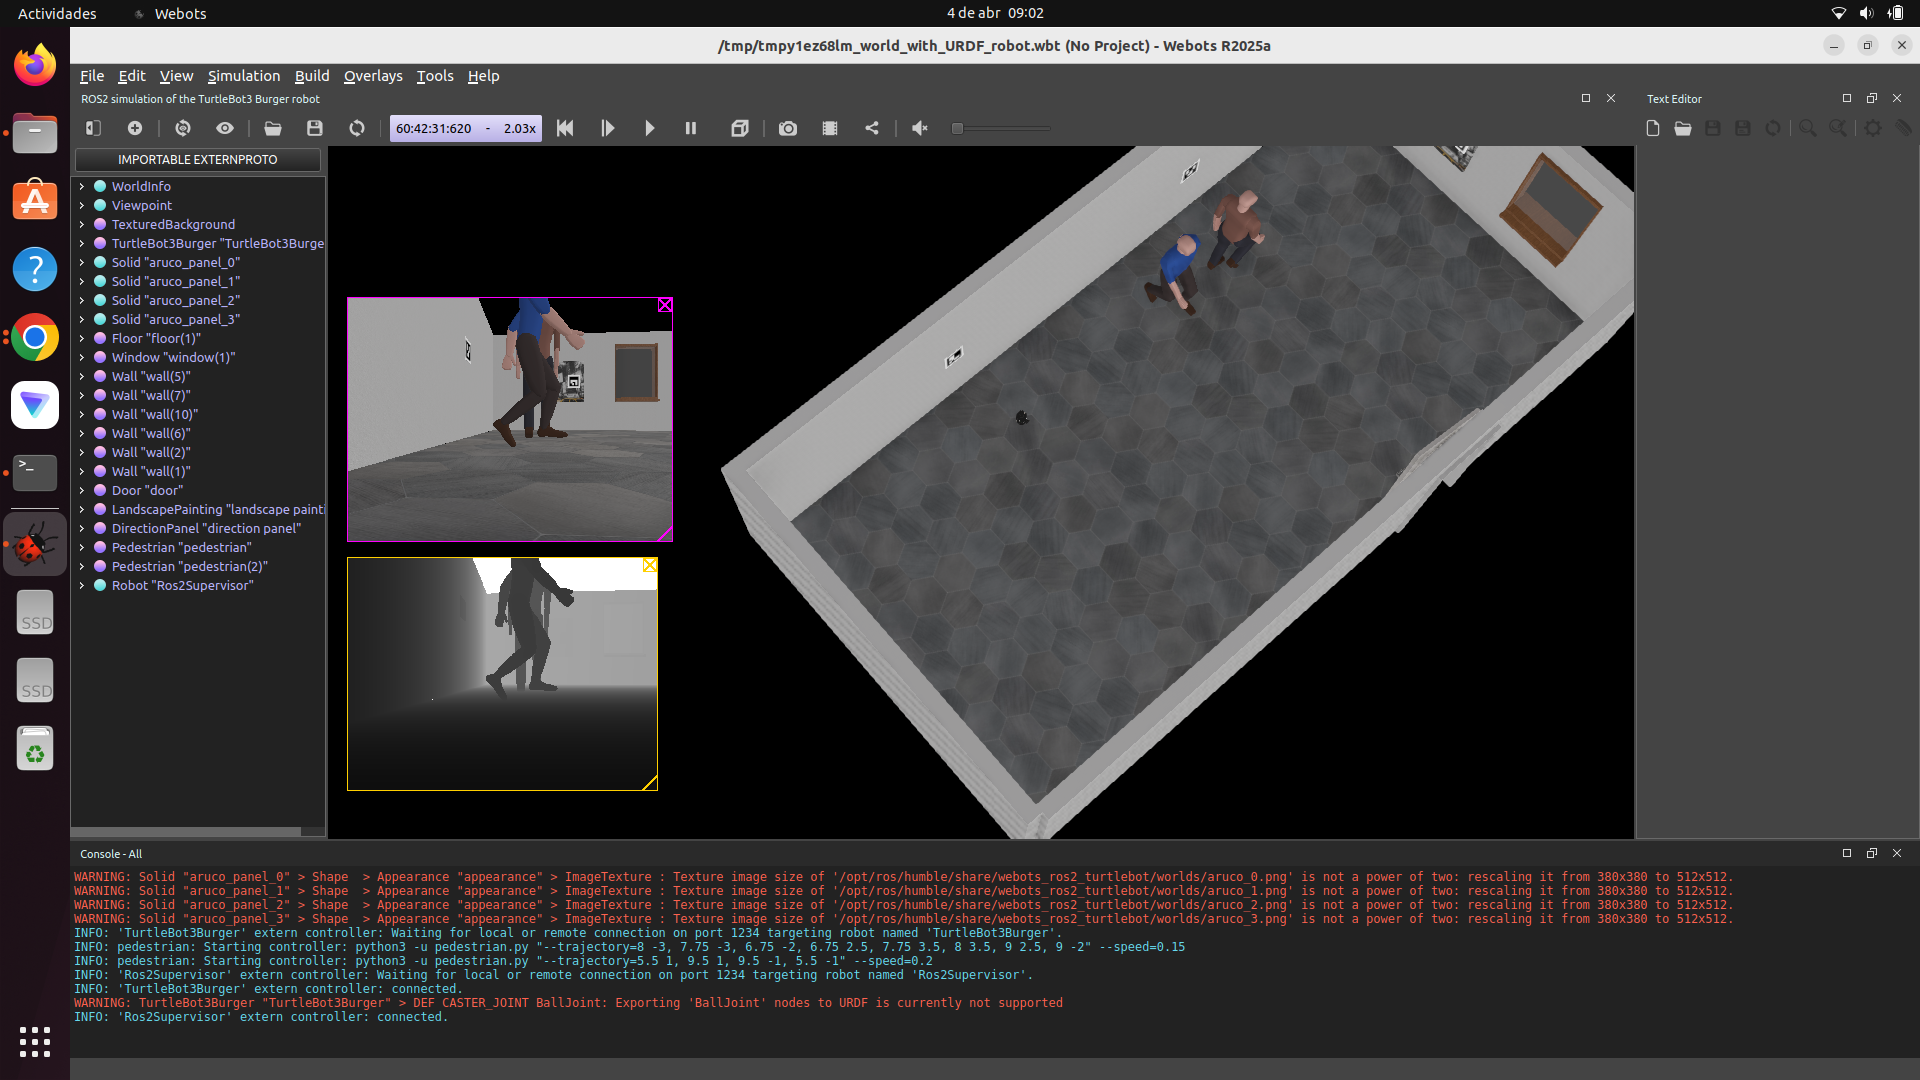
\includegraphics[width=\linewidth,height=0.82\textheight,keepaspectratio]{sim_04_debug.png}
  \caption{Debug visualisation during tracking. The top-left panel shows the
           RGB debug image published on
           \texttt{/person\_\allowbreak follower/\allowbreak debug\_image}: a magenta bounding box
           surrounds the tracked person, confirming identity lock. The
           bottom-left panel shows the corresponding \texttt{32FC1} depth
           image from the range finder, where the pedestrian silhouette is
           clearly visible against the background. The Webots 3-D view (right)
           confirms the robot is positioned behind and aligned with the target.}
  \label{fig:sim_debug}
\end{figure}

% ========================================================================
\section{Trajectory Analysis}
\label{sec:trajectories}

This section evaluates the behaviour of the system by plotting, in the Webots
world frame, the path travelled by the robot together with the ground-truth
paths of the pedestrians and the target position estimated by the perception
pipeline.

\subsection{Data Sources}

Three independent sources of trajectory data are combined:

\begin{itemize}
  \item \textbf{Robot trajectory.} The wheel odometry published on
    \texttt{/odom} provides the robot pose throughout the run.
  \item \textbf{Perceived target trajectory.} The node publishes the fused
    measurement and the Kalman estimate of the target on the topics
    \texttt{/person\_\allowbreak follower/\allowbreak target\_\allowbreak measurement} and
    \texttt{/person\_\allowbreak follower/\allowbreak target\_\allowbreak estimate} (both of type
    \texttt{geometry\_\allowbreak msgs/\allowbreak PointStamped}). Recording these together with
    \texttt{/odom} makes the rosbag self-contained for the analysis.
  \item \textbf{Pedestrian ground truth.} The Webots \texttt{Pedestrian}
    nodes follow deterministic way-point lists declared in the \texttt{.wbt}
    world file through the \texttt{-{}-trajectory} controller argument. These
    way-points are the exact ground-truth paths and are parsed directly from
    the world file.
\end{itemize}

\subsection{Reference Frames}

The \texttt{/odom} topic is expressed in the \texttt{odom} frame, whose origin
coincides with the robot start pose, whereas the pedestrian way-points are
given in the Webots world frame. To overlay both, the odometry samples are
transformed into world coordinates with the rigid transformation

\begin{equation}
  \begin{pmatrix} x_w \\ y_w \end{pmatrix} =
  R(\theta_0)
  \begin{pmatrix} x_o \\ y_o \end{pmatrix} +
  \begin{pmatrix} x_0 \\ y_0 \end{pmatrix},
  \qquad
  R(\theta_0) =
  \begin{pmatrix} \cos\theta_0 & -\sin\theta_0 \\
                  \sin\theta_0 &  \cos\theta_0 \end{pmatrix}
\end{equation}

where $(x_0,\,y_0,\,\theta_0)$ is the robot start pose read from the
\texttt{.wbt} file. For \texttt{turtlebot3\_\allowbreak burger\_\allowbreak pedestrian\_\allowbreak simple.wbt}
this is $(x_0,y_0) = (6.75,\,-3.00)$~m and $\theta_0 = \pi/2$~rad. The same
transformation is applied to the target topics, since they are computed from
the robot odometry and therefore share the \texttt{odom} frame.

\subsection{Analysis Script}

All figures in this section are produced by the script
\texttt{report/plot\_trajectories.py}, which reads a recorded rosbag, parses
the world file, applies the transformation above and renders the plots with
Matplotlib:

\begin{verbatim}
# from the report/ directory, with ROS 2 sourced
python3 plot_trajectories.py --bag rosbags/exp_01
\end{verbatim}

\noindent The procedure to record the rosbag is described in
Appendix~\ref{app:rosbags}.

\subsection{Results}

A continuous experiment of 10.3~minutes (618~s) was recorded with the robot
configured to follow pedestrian~1. During the run the perception pipeline
produced 384 valid target detections --- an average rate of only 0.62~Hz. The
mean interval between detections was 1.6~s and the longest single loss of the
target lasted 76~s. This low detection rate is the dominant factor in the
results below; its cause is analysed in Section~\ref{sec:limitations}.

\begin{figure}[htbp]
  \centering
  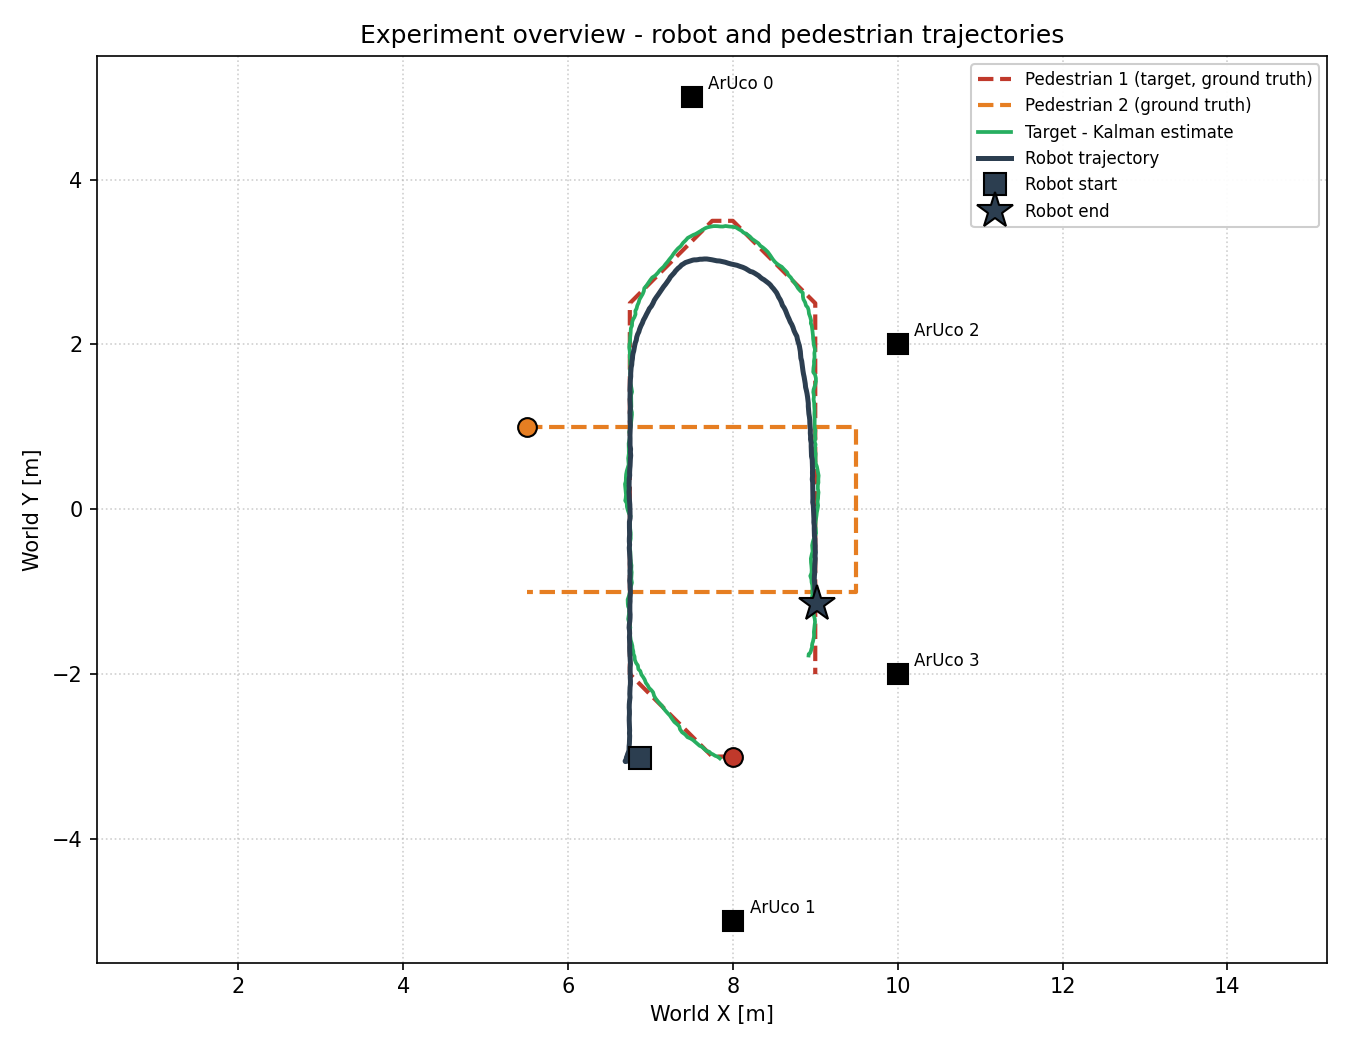
\includegraphics[width=\linewidth,height=0.82\textheight,keepaspectratio]{traj_overview.png}
  \caption{Global overview of the recorded experiment. The robot trajectory
           is shown in dark blue and the Kalman estimate of the target in
           green; the green line is broken wherever the target was lost. The
           ground-truth pedestrian paths are dashed and the four ArUco panel
           positions are marked for reference.}
  \label{fig:traj_overview}
\end{figure}

Figure~\ref{fig:traj_overview} shows that the robot stayed largely within the
central region of the room instead of following pedestrian~1 around its full
loop. Because the target was detected only intermittently, the robot spent a
large fraction of the run in the search behaviour (Mode~3), turning in place
to re-acquire the pedestrian. The Kalman estimate appears as a set of
disconnected segments: each gap corresponds to an interval with no detection.

\begin{figure}[htbp]
  \centering
  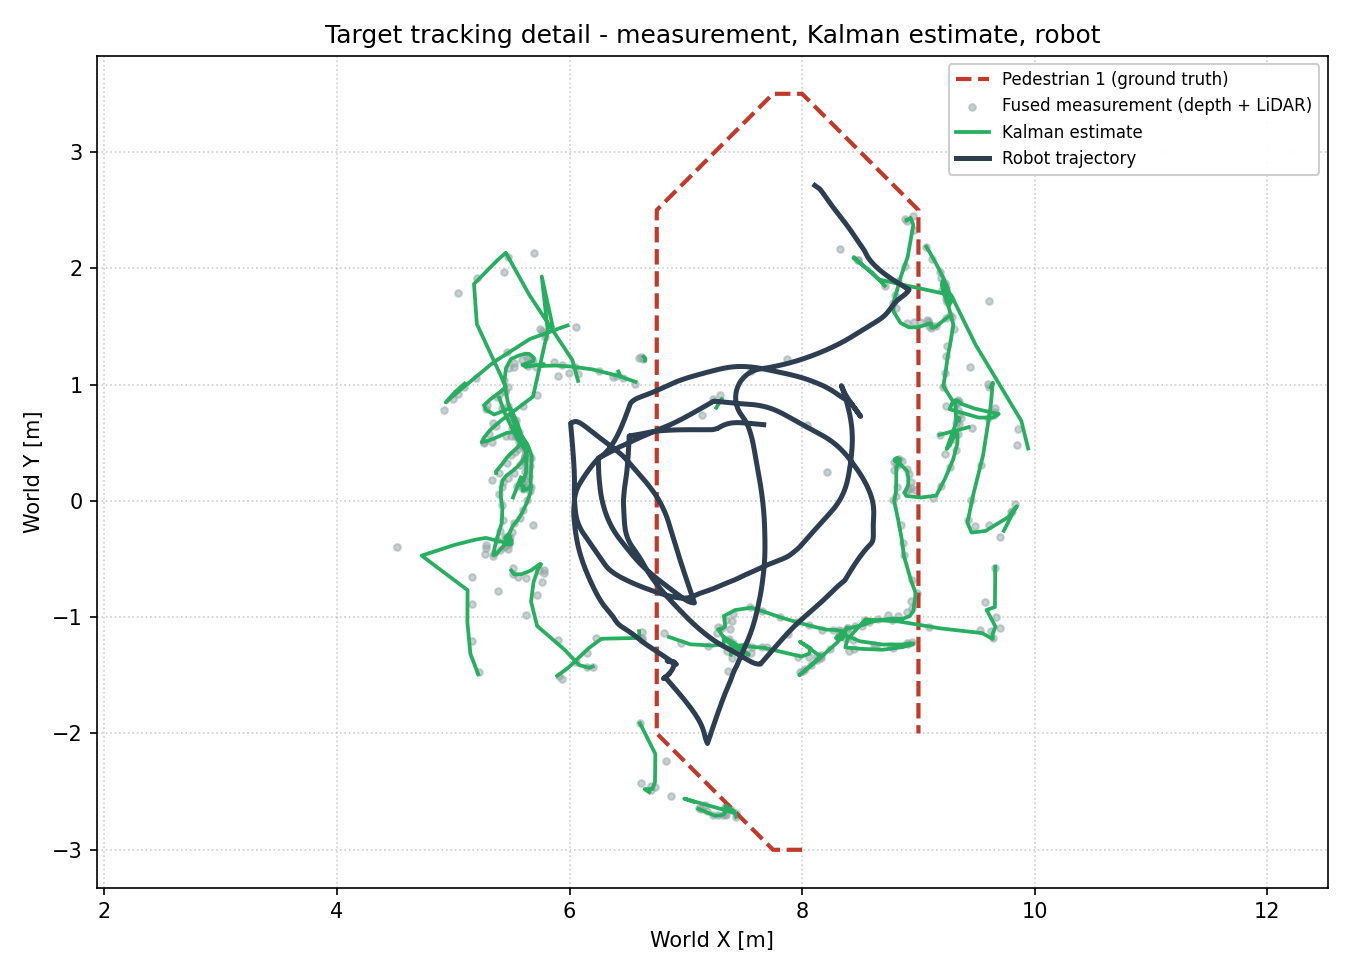
\includegraphics[width=\linewidth,height=0.82\textheight,keepaspectratio]{traj_following.png}
  \caption{Detail of the target tracking: the fused depth\,+\,LiDAR
           measurements (grey dots), the Kalman estimate (green, broken at
           detection losses) and the robot trajectory (dark blue), against the
           ground-truth path of pedestrian~1 (red dashed).}
  \label{fig:traj_following}
\end{figure}

Figure~\ref{fig:traj_following} shows that, whenever a detection is available,
the fused measurement and the Kalman estimate fall close to the ground-truth
pedestrian path: the perception pipeline is accurate. The limitation is not
accuracy but \emph{update rate} --- the estimate is not refreshed often enough
to keep the controller continuously informed.

\begin{figure}[htbp]
  \centering
  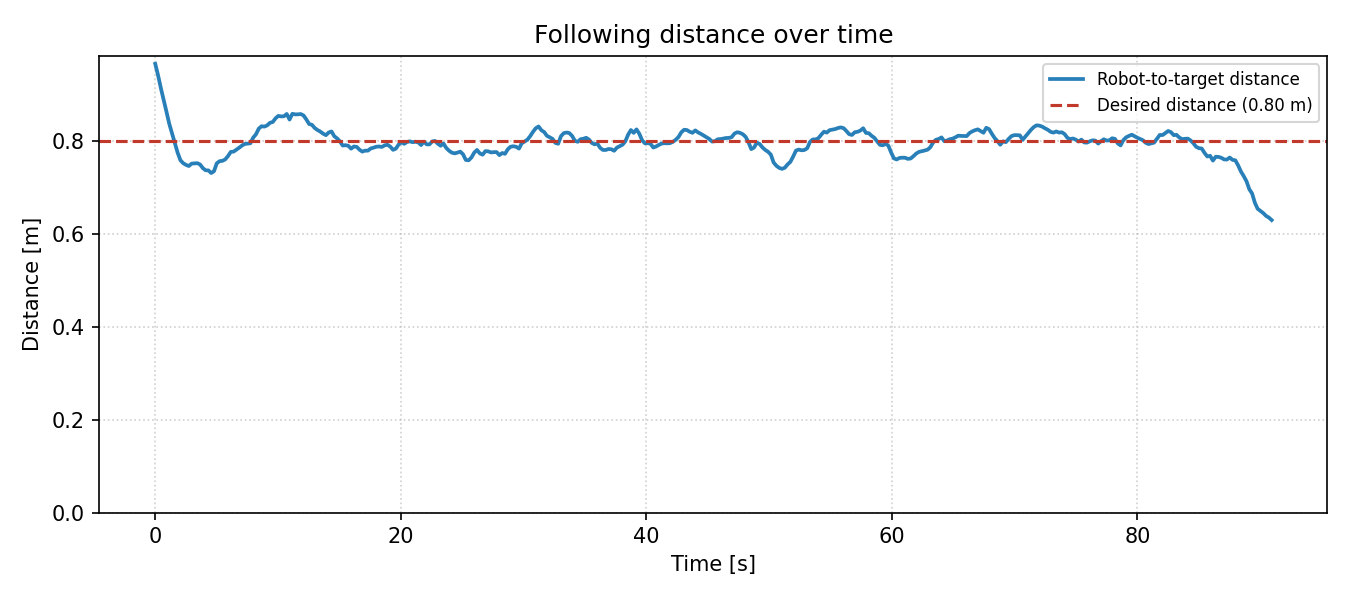
\includegraphics[width=\linewidth,height=0.82\textheight,keepaspectratio]{traj_distance.png}
  \caption{Robot-to-target distance, evaluated at each detection. The line is
           broken where the target was lost for more than 2~s. The desired
           following distance of 0.8~m is the red dashed line.}
  \label{fig:traj_distance}
\end{figure}

Figure~\ref{fig:traj_distance} quantifies the following performance. The
robot-to-target distance ranged from 0.56~m to 2.42~m, with a mean of 1.43~m
and a median of 1.38~m --- well above the desired 0.8~m. Only 27\% of the
detections fell within the 0.5--1.1~m band around the set-point, although the
robot never came dangerously close to the pedestrian (no detection below
0.4~m). The frequent breaks in the line are the detection losses already
apparent in the previous figures.

\subsection{Discussion and Limitations}
\label{sec:limitations}

The experiment was run on a laptop \emph{without a dedicated GPU}. Running
YOLOv8 inference on the CPU is the bottleneck of the whole pipeline: it caps
the perception update rate at roughly 0.6~Hz, so the robot is effectively
blind for about 1.6~s between detections. At a walking speed of 0.15~m/s the
pedestrian moves around 0.25~m in that interval, and after a longer loss it
can leave the camera field of view entirely, forcing the robot into the
search behaviour. This is the direct cause of the large distance error and
the fragmented estimate reported above.

This is a \emph{hardware} limitation rather than a flaw in the design. When a
detection is available the fused estimate is accurate
(Figure~\ref{fig:traj_following}), and the sensor-fusion, Kalman-filtering and
control logic behave as intended. Continuous following at the designed 0.8~m
gap requires a perception rate on the order of 10--30~Hz; on this pipeline
that means GPU-accelerated inference. Lighter alternatives --- a smaller
detector, a lower camera resolution, or running YOLO less often while relying
more on the Kalman prediction between frames --- would also raise the
effective update rate. Re-running the same experiment on a GPU-equipped
machine is expected to bring the following distance close to the 0.8~m
set-point.


\section{Conclusion}

The person-follower node integrates five complementary techniques for person tracking
in a cluttered indoor simulation:

\begin{enumerate}
  \item \textbf{YOLOv8 + BoTSORT} provide reliable short-term person
    detection and identity maintenance.
  \item \textbf{HSV Re-ID} recovers the correct target after occlusions using
    appearance similarity.
  \item \textbf{Sensor fusion} (depth + LiDAR) produces a more robust
    distance estimate than either sensor alone.
  \item \textbf{Kalman filtering} in world coordinates smooths noisy
    measurements and enables short-horizon dead-reckoning navigation.
  \item \textbf{ArUco markers} provide an absolute position reference that
    can correct odometry drift over long sessions.
\end{enumerate}

The modular callback architecture makes it straightforward to tune individual
subsystems independently and to extend the pipeline with additional sensors or
more sophisticated controllers.

The trajectory analysis of Section~\ref{sec:trajectories} showed, however,
that on CPU-only hardware the achievable perception rate --- not the control
or fusion logic --- becomes the factor that limits following performance.
GPU-accelerated inference is therefore recommended for real-time operation.

% ========================================================================
\newpage
\addcontentsline{toc}{section}{References}
\begin{thebibliography}{99}

\bibitem{ros2}
S.~Macenski, T.~Foote, B.~Gerkey, C.~Lalancette, and W.~Woodall,
``Robot Operating System 2: Design, architecture, and uses in the wild,''
\emph{Science Robotics}, vol.~7, no.~66, eabm6074, 2022.

\bibitem{webots}
O.~Michel,
``Webots: Professional Mobile Robot Simulation,''
\emph{International Journal of Advanced Robotic Systems}, vol.~1, no.~1,
pp.~39--42, 2004.

\bibitem{turtlebot3}
R.~Amsters and P.~Slaets,
``Turtlebot 3 as a Robotics Education Platform,''
in \emph{Robotics in Education (RiE 2019)}, Advances in Intelligent Systems
and Computing, vol.~1023.\ Cham: Springer, 2020, pp.~170--181.

\bibitem{opencv}
G.~Bradski,
``The OpenCV Library,''
\emph{Dr.\ Dobb's Journal of Software Tools}, 2000.

\bibitem{numpy}
C.~R.~Harris \emph{et al.},
``Array programming with NumPy,''
\emph{Nature}, vol.~585, pp.~357--362, 2020.

\bibitem{yolo}
J.~Redmon, S.~Divvala, R.~Girshick, and A.~Farhadi,
``You Only Look Once: Unified, Real-Time Object Detection,''
in \emph{Proc.\ IEEE Conf.\ on Computer Vision and Pattern Recognition
(CVPR)}, 2016, pp.~779--788.

\bibitem{yolov8}
G.~Jocher, A.~Chaurasia, and J.~Qiu,
``Ultralytics YOLOv8,'' version~8.0.0, 2023. [Online]. Available:
\url{https://github.com/ultralytics/ultralytics}

\bibitem{sort}
A.~Bewley, Z.~Ge, L.~Ott, F.~Ramos, and B.~Upcroft,
``Simple Online and Realtime Tracking,''
in \emph{Proc.\ IEEE Int.\ Conf.\ on Image Processing (ICIP)}, 2016,
pp.~3464--3468.

\bibitem{botsort}
N.~Aharon, R.~Orfaig, and B.-Z.~Bobrovsky,
``BoT-SORT: Robust Associations Multi-Pedestrian Tracking,''
arXiv:2206.14651, 2022.

\bibitem{comaniciu}
D.~Comaniciu, V.~Ramesh, and P.~Meer,
``Kernel-Based Object Tracking,''
\emph{IEEE Transactions on Pattern Analysis and Machine Intelligence},
vol.~25, no.~5, pp.~564--577, 2003.

\bibitem{arras}
K.~O.~Arras, O.~Mart\'{\i}nez~Mozos, and W.~Burgard,
``Using Boosted Features for the Detection of People in 2D Range Data,''
in \emph{Proc.\ IEEE Int.\ Conf.\ on Robotics and Automation (ICRA)}, 2007,
pp.~3402--3407.

\bibitem{aruco}
S.~Garrido-Jurado, R.~Mu\~{n}oz-Salinas, F.~J.~Madrid-Cuevas, and
M.~J.~Mar\'{\i}n-Jim\'{e}nez,
``Automatic generation and detection of highly reliable fiducial markers
under occlusion,''
\emph{Pattern Recognition}, vol.~47, no.~6, pp.~2280--2292, 2014.

\bibitem{aruco2}
F.~J.~Romero-Ramirez, R.~Mu\~{n}oz-Salinas, and R.~Medina-Carnicer,
``Speeded up detection of squared fiducial markers,''
\emph{Image and Vision Computing}, vol.~76, pp.~38--47, 2018.

\bibitem{kalman}
R.~E.~Kalman,
``A New Approach to Linear Filtering and Prediction Problems,''
\emph{Journal of Basic Engineering}, vol.~82, no.~1, pp.~35--45, 1960.

\bibitem{barshalom}
Y.~Bar-Shalom, X.-R.~Li, and T.~Kirubarajan,
\emph{Estimation with Applications to Tracking and Navigation}.
New York: John Wiley \& Sons, 2001.

\end{thebibliography}

% ========================================================================
\newpage
\appendix

\section{Running the Simulation}
\label{app:running}

This appendix gives the complete procedure to build and run the
person-follower in simulation. It assumes Ubuntu~22.04 with
ROS~2~Humble~\cite{ros2} and Webots~R2025a~\cite{webots} already installed,
with Webots extracted to \texttt{\$HOME/webots-R2025a}.

\subsection{Prerequisites}

Install the TurtleBot3 packages for \texttt{webots\_ros2} and the Python
dependencies used by the perception node:

\begin{verbatim}
sudo apt update
sudo apt install ros-humble-webots-ros2-turtlebot ros-humble-cv-bridge
pip3 install ultralytics opencv-contrib-python numpy
\end{verbatim}

\subsection{Build the Package}

\begin{verbatim}
mkdir -p ~/ros2_ws/src
cd ~/ros2_ws/src
git clone https://github.com/mr7g0l/person_follower.git
cd ~/ros2_ws
source /opt/ros/humble/setup.bash
colcon build --symlink-install
\end{verbatim}

\subsection{Generate the ArUco Textures}

The marker PNG textures are already included in the repository. To regenerate
them (for example after changing the marker dictionary), run:

\begin{verbatim}
cd ~/ros2_ws/src/person_follower
python3 webots/generate_aruco_markers.py
\end{verbatim}

\subsection{Install the World Files}

Copy the world files \emph{and} the ArUco textures into the
\texttt{webots\_ros2\_turtlebot} package, so that Webots can locate the
texture images referenced by the world:

\begin{verbatim}
WORLDS=/opt/ros/humble/share/webots_ros2_turtlebot/worlds
sudo cp ~/ros2_ws/src/person_follower/webots/*.wbt       $WORLDS/
sudo cp ~/ros2_ws/src/person_follower/webots/aruco_*.png $WORLDS/
\end{verbatim}

\subsection{Launch the System}

The system runs in three terminals. In every terminal, ROS~2 must be sourced
first.

\textbf{Terminal 1 --- perception and control node:}
\begin{verbatim}
source /opt/ros/humble/setup.bash
source ~/ros2_ws/install/setup.bash
export ROS_LOCALHOST_ONLY=1
ros2 run person_follower person_follower
\end{verbatim}

\textbf{Terminal 2 --- Webots simulator:}
\begin{verbatim}
export WEBOTS_HOME=~/webots-R2025a
source /opt/ros/humble/setup.bash
export ROS_LOCALHOST_ONLY=1
ros2 launch webots_ros2_turtlebot robot_launch.py \
  world:=turtlebot3_burger_pedestrian_simple.wbt
\end{verbatim}

\textbf{Terminal 3 --- RViz visualisation (optional):}
\begin{verbatim}
source /opt/ros/humble/setup.bash
export ROS_LOCALHOST_ONLY=1
rviz2 -d ~/ros2_ws/src/person_follower/webots/config.rviz
\end{verbatim}

Once Webots is running, the robot locks onto the nearest pedestrian and starts
following it. The annotated camera stream is published on
\texttt{/person\_\allowbreak follower/\allowbreak debug\_image} and can be inspected with
\texttt{rqt\_image\_view}.

% ========================================================================
\section{Recording and Replaying Experiments}
\label{app:rosbags}

To document an experiment in a reproducible way, the relevant ROS~2 topics are
recorded into a rosbag.

\subsection{Recording}

With the simulation running (Appendix~\ref{app:running}), start the recording
in a new terminal:

\begin{verbatim}
cd ~/ros2_ws/src/person_follower/webots
./record_experiment.bash exp_01
\end{verbatim}

The helper script \texttt{record\_experiment.bash} stores the bag under
\texttt{report/\allowbreak rosbags/\allowbreak exp\_01\_\allowbreak<timestamp>} and records the topics
\texttt{/odom}, \texttt{/cmd\_vel}, \texttt{/scan},
\texttt{/person\_\allowbreak follower/\allowbreak target\_\allowbreak measurement} and
\texttt{/person\_\allowbreak follower/\allowbreak target\_\allowbreak estimate}. Press \texttt{Ctrl-C} to stop.
The contents of a bag can be inspected with:

\begin{verbatim}
ros2 bag info report/rosbags/exp_01_<timestamp>
\end{verbatim}

\subsection{Replaying}

A recorded experiment can be played back so that the trajectories, the laser
scan and the velocity commands are republished on their original topics:

\begin{verbatim}
source /opt/ros/humble/setup.bash
export ROS_LOCALHOST_ONLY=1
ros2 bag play report/rosbags/exp_01_<timestamp>
\end{verbatim}

While the bag is playing, RViz (Appendix~\ref{app:running}) can be used to
visualise the laser scan and the robot motion.

\subsection{Generating the Trajectory Plots}

The figures of Section~\ref{sec:trajectories} are produced from the recorded
bag with:

\begin{verbatim}
cd ~/ros2_ws/src/person_follower/report
pip3 install matplotlib numpy
python3 plot_trajectories.py --bag rosbags/exp_01_<timestamp>
\end{verbatim}

This writes \texttt{traj\_overview.png}, \texttt{traj\_following.png} and
\texttt{traj\_distance.png} into the \texttt{report/} directory and prints the
summary statistics of the run.

\subsection{Sharing the Rosbags}

Recorded rosbags are too large to be stored in the Git repository (the
\texttt{report/rosbags/} directory is therefore excluded in
\texttt{.gitignore}). They are instead uploaded to Google Drive with link
sharing enabled, and the link is added here and to the project
\texttt{README}:

\begin{center}
\url{https://drive.google.com/drive/folders/1HjiBTtxrNCbCuHkJ0b46jUU2g8fwfBa-?usp=drive_link}
\end{center}

\noindent To reproduce the analysis, download the bag from that link and run
the commands above on the downloaded directory.


\end{document}
